% !TeX encoding = UTF-8

\chapter{IMPLEMENTAÇÃO DAS TÉCNICAS}\label{ch:implementacao}
Este capítulo tem como objetivo apresentar, de forma mais detalhada, todo o processo de implementação realizado no presente trabalho, com o intuito de alcançar os objetivos especificados no Capítulo 1.

\section{REALIZAÇÃO DA COLETA DE DADOS}
Tendo em vista as ferramentas necessárias para realizar à coleta das séries temporais que serão utilizadas para o treinamento e testes da RNA, foi desenvolvido um método de automatização de aquisição dos \textit{DataFrames} das ações que serão coletadas para a análise.

Inicialmente, foi criada uma interface em Python que contém a assinatura do método que as classes das empresas deverão implementar. Após isso, foram criadas as classes para as respectivas empresas, definidas no Seção 4.2. Para exemplificar o que está sendo exposto, o Código 3 demonstra, de forma mais intuituva, a implementação do atual procedimento.
\codigoPython\
\lstinputlisting[label=cod:exempla-coleta, caption=Implementação da interface Empresa em Python]{src/empresa.py}

Analisando este código, pode-se observar o desenvolvimento da interface "Empresa"\, e da classe "Apple", que implementa esta interface através do parâmetro (Empresa) em sua definição. Também é possível observar, na classe Apple, a implementação do método construtor "\_\_init\_\_"\, que contém seu respectivo nome e código, necessário para realizar a busca. O método "executa\_busca", por sua vez, faz uma chamada ao objeto que realizará a coleta das respectivas ações, passando seus parâmetros como valor. O Código 4 ilustra a implementação do objeto de busca.

\lstinputlisting[language=Python, label=cod-crawler, caption=Implementação do objeto Crawler que realiza a busca das ações]{src/crawler.py}

O Código 4 utiliza a biblioteca pandas para realizar a coleta das ações. Pode-se observar que o método construtor "\_\_init\_\_"\, recebe o nome e o código da empresa que faz a chamada de sua instância. Também é possível analisar o método "executa\_busca"\, implementado, que realiza a chamada da função "web.DataReader"\,
passando quatro parâmetros, sendo eles:
\begin{enumerate}
\item Código da empresa;
\item API que será realizada a busca;
\item Data de inicial da coleta;
\item Data final da coleta.
\end{enumerate}

Após a realização da requisição, a API retorna um arquivo com as ações entre as respectivas datas, no formato especificado na Seção 4.4.2, formando assim, o \textit{DataFrame} inicial das empresas. Este procedimento foi realizado para todas as empresas que são analisadas neste trabalho.

Posteriormente, são analisadas as séries específicas de cada empresa, através de seus valores diários de abertura. O período coletado foi de 09/04/2001 a 31/08/2017.

Iniciando por ordem alfabética, as ações da Amazon contém os valores mais altos dentre as empresas estudadas. No período coletado, seu valor de abertura apresentou um mínimo de 5,91 e um máximo de 1069,55 dólares Americanos (USD), evidenciando seu crescimento e valorização. O Gráfico 2 representa o comportamento desta série.
\begin{grafico}[h]
	\centering
	\centerline{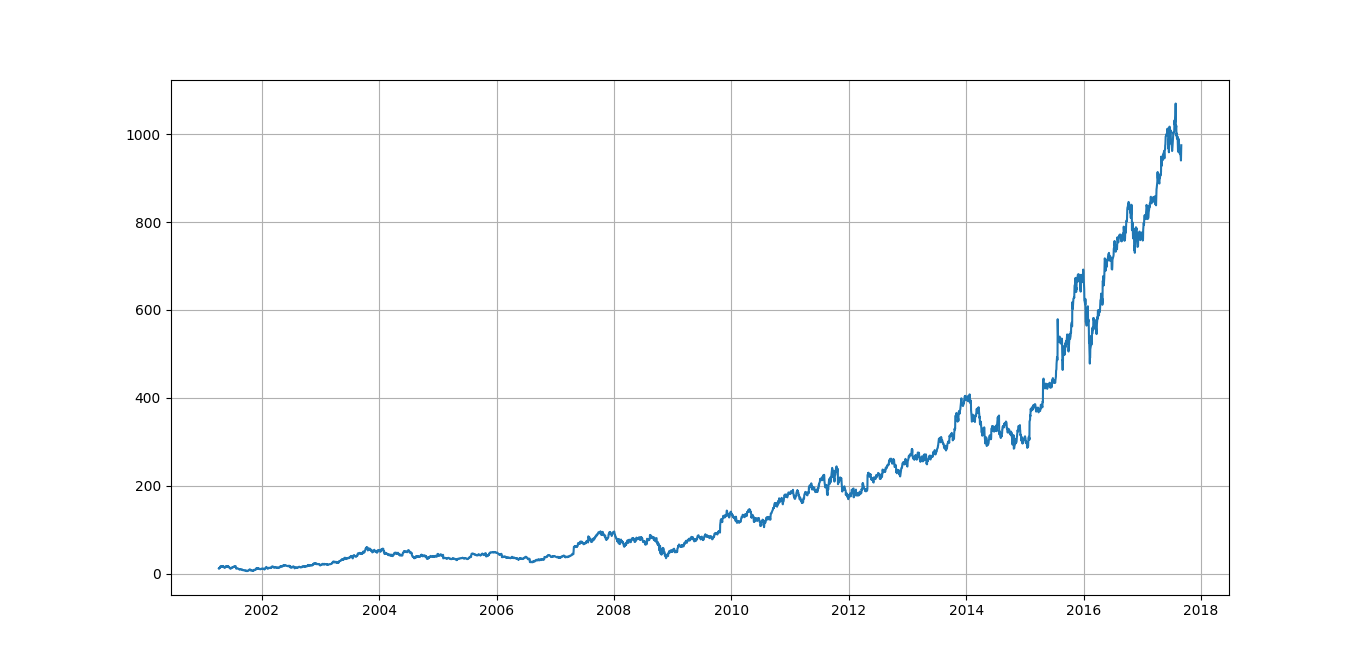
\includegraphics[scale=4]{amazon_coletado}}
	\caption{Valores de abertura das ações da Amazon}
	\fonte{Elaborado pelo autor}
	\label{exec-amazon-coleta}
\end{grafico}

As ações da Apple contam com seus valores mais constantes, sem grande ascenção se comparada a Amazon. Seu valor de abertura apresentou um mínimo de 0,93 e um máximo de 163,80 USD. O Gráfico 3 representa o comportamento desta série.

As ações da Cisco, Intel e Microsoft possuem os valores mais equilibrados dentre as empresas selecionadas. O valor de abertura mínimo apresentado pela Cisco, no período coletado, foi de 8,45 enquanto seu valor máximo foi de 34,46 USD. Já a Intel, apresentou um valor um mínimo de 12,17 e um máximo de 38,25 USD. Por fim, a Microsoft também apresentou uma série bem equilibrada no período coletado, variando entre um valor mínimo de 15,20 e um máximo de 74,34 USD. Os Gráficos 4, 5 e 6 mostram, de forma mais intuitiva, as ações da Cisco, Intel e Microsoft, respectivamente. 	
\begin{grafico}[h]
	\centering
	\centerline{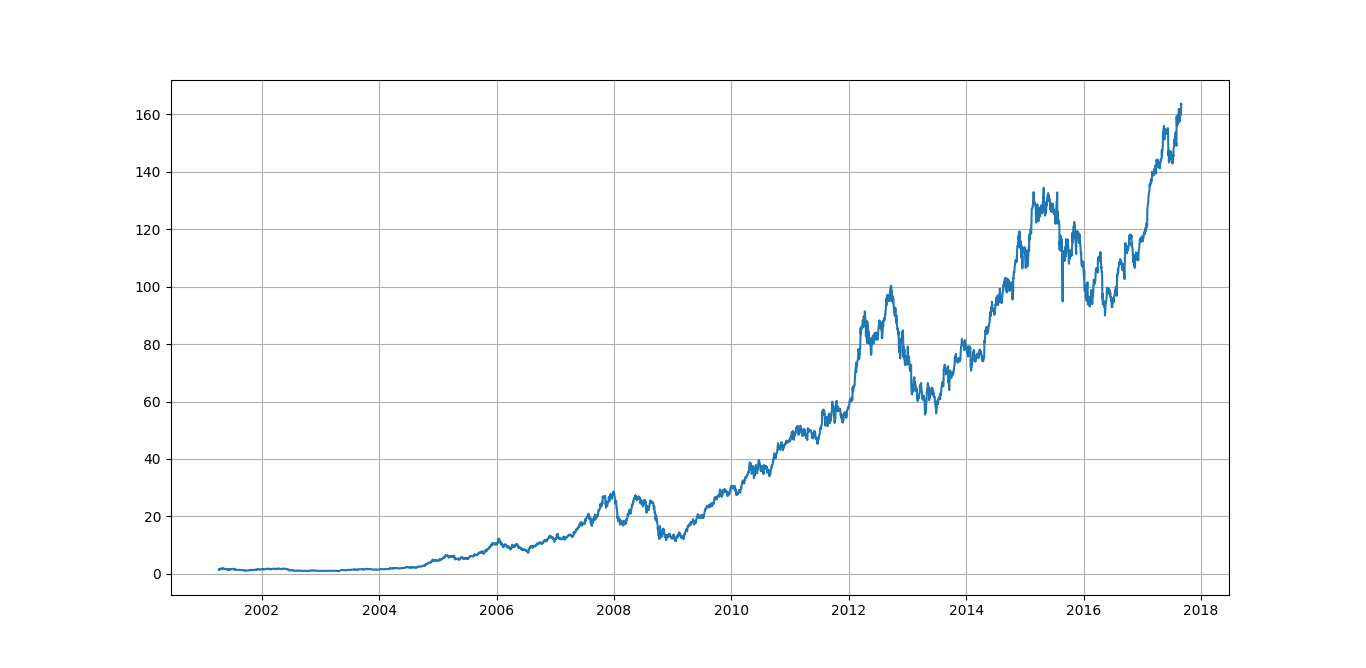
\includegraphics[scale=4]{apple_coletado}}
	\caption{Valores de abertura das ações da Apple}
	\fonte{Elaborado pelo autor}
	\label{exec-apple-coleta}
\end{grafico}

\begin{grafico}[h]
	\centering
	\centerline{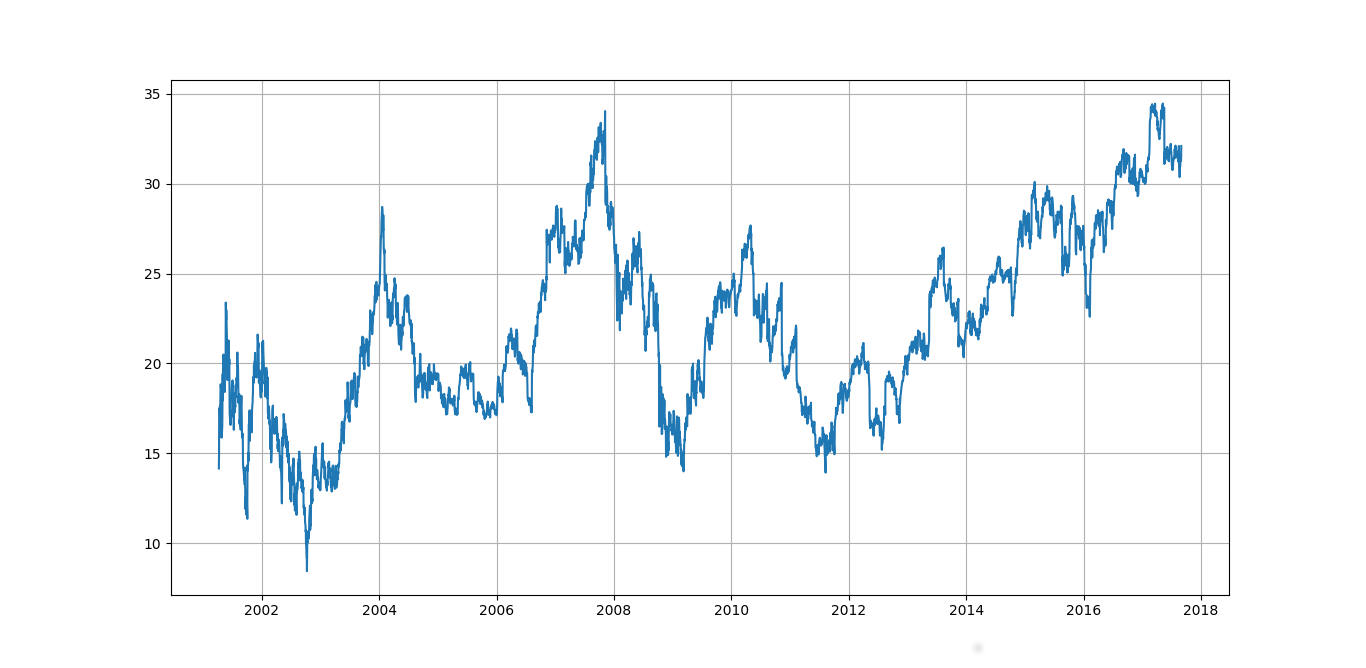
\includegraphics[scale=4]{cisco_coletado}}
	\caption{Valores de abertura das ações da Cisco}
	\fonte{Elaborado pelo autor}
	\label{exec-cisco-coleta}
\end{grafico}
 
\begin{grafico}[h]
	\centering
	\centerline{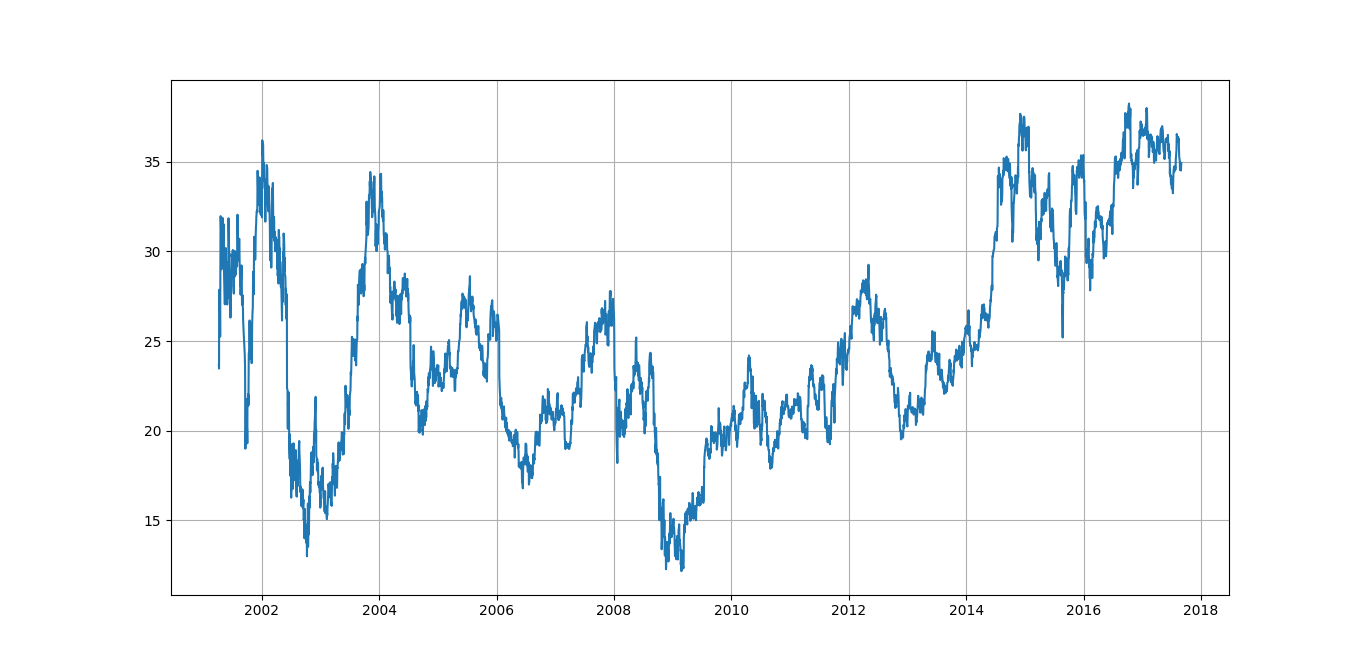
\includegraphics[scale=4]{intel_coletado}}
	\caption{Valores de abertura das ações da Intel}
	\fonte{Elaborado pelo autor}
	\label{exec-intel-coleta}
\end{grafico}

\begin{grafico}[h]
	\centering
	\centerline{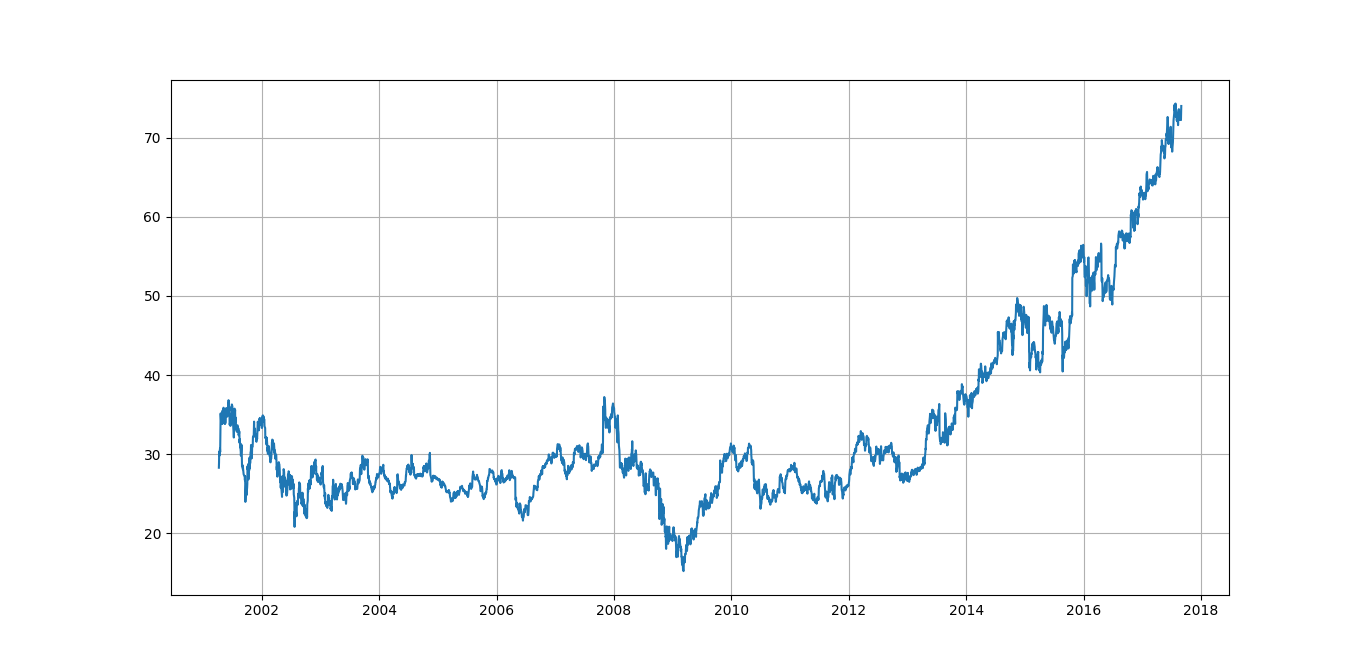
\includegraphics[scale=4]{microsoft_coletado}}
	\caption{Valores de abertura das ações da Microsoft}
	\fonte{Elaborado pelo autor}
	\label{exec-microsoft-coleta}
\end{grafico}

\clearpage
\section{EXPLORANDO O \textit{DATAFRAME}}
O refinamento do modelo de dados coletado é de suma importância para agregar valor às informações do \textit{DataFrame} de cada empresa. Como especificado na Seção 4.3.1, é necessário calcular alguns indicadores técnicos, que são consideradas informações expressivas que influenciam diretamente nos valores das ações.

Para desenvolver o cálculo das médias móveis de 10 e 26 dias, foi formada uma equação levando em consideração o exposto na Seção 4.3.1, o que proporciona de uma forma mais clara como realizar a implementação do algoritmo. A equação (5.1) demonstra este procedimento:
\begin{equation}\label{eq:MMS}
M_t = \dfrac{Z_t + Z_{t-1} + \dots + Z_{t-k+1}}{k},
\end{equation}
onde k é a quantidade de dias que se deseja calcular a média, t é o índice iterador da sequência que está sendo calculada e Z é o valor de fechamento da ação no momento t. A partir disto, foi desenvolvida uma função que realiza este cálculo. O Código 5 ilustra com detalhes esta implementação. 
\lstinputlisting[language=Python, label=cod-media-movel, caption=Implementação da função que realiza o cálculo da média móvel]{src/media-movel.py}

O Código 5 recebe como parâmetro o índice do \textit{DataFrame} e a quantidade de dias que se deseja calcular a média móvel. O algoritmo encontra este índice e, a partir disso, faz um incremento com o valor de fechamento. Após atingir o limite de incrementos necessários, levando em consideração a quantidade de dias, realiza a divisão e salva o valor em uma nova coluna do \textit{DataFrame}.

Já para o cálculo do indicador técnico MACD, o mesmo é realizado de forma mais simples com o auxílio da biblioteca pandas. O Código 6 cria uma nova coluna ao \textit{DataFrame} e realiza o cálculo da diferença, utilizando a função "sub", entre as duas médias móveis.
\lstinputlisting[language=Python, label=cod-media-movel, caption=Implementação da função que realiza o cálculo do MACD]{src/macd.py}

Finalizada a etapa de cálculo dos indicadores técnicos, todos os parâmetros necessários para iniciar a implementação da RNA, especificados no Capítulo 4, foram coletados e estruturados. A Figura 13 ilustra exatamente como ficou o \textit{DataFrame} após a inserção das novas colunas.
\begin{figure}[h]
	\centering
	\fbox{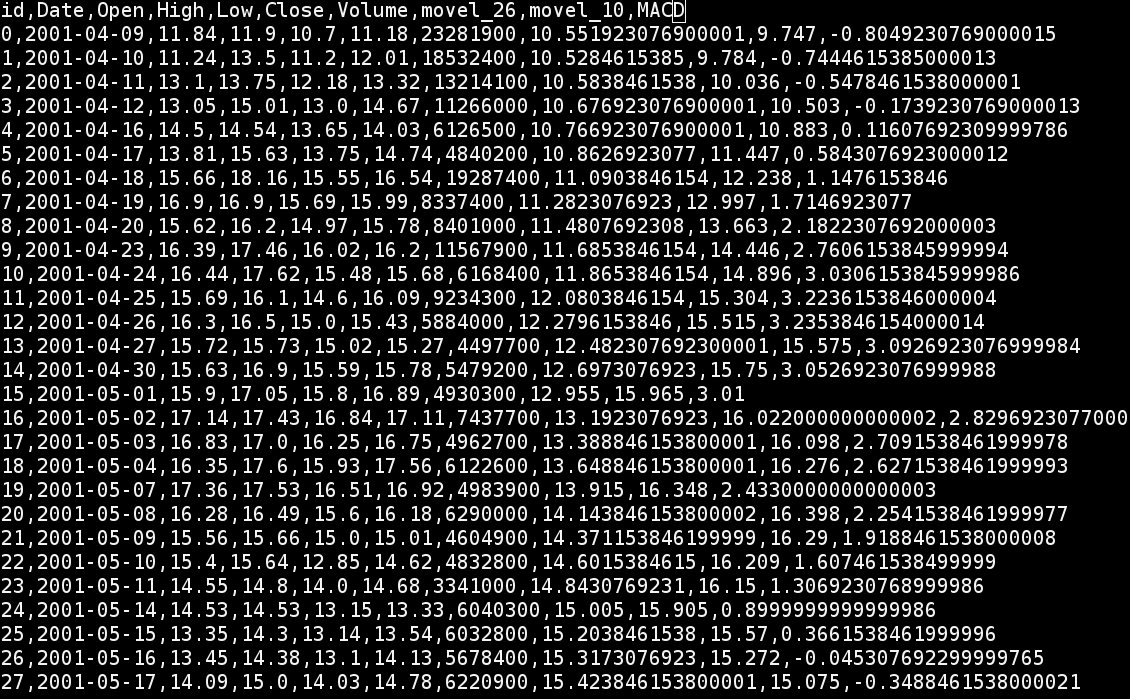
\includegraphics[width=0.8\textwidth, scale=0.5]{dados_formatados}}
	\caption{Exemplo do \textit{DataFrame} com os dados atualizados}
	\fonte{Elaborado pelo autor}
	\label{exec-dados-formatados}	
\end{figure}

\section{NORMALIZANDO OS DADOS}
Segundo \citeonline{Luiz}, o evento que antecede a etapa de treinamento de uma RNA é o processo de normalização dos dados de entrada e saída. Como o modelo proposto trabalha com a função de ativação sigmóide, detalhada na Seção 3.3.2, os dados devem ser normalizados entre um intervalo de [0,1]. A normalização consiste em adaptar uma base de dados com valores disintos, o que se aplica à realidade do presente trabalho, onde os valores das ações contam com intervalos de grande oscilação.

Considerando estas informações, duas equações foram especificadas para realizar a normalização e a desnormalização dos dados, com o objetivo de treinar a rede de forma mais eficaz, sendo elas:
\begin{equation}\label{eq:eq-normalizacao}
L_n = (L_o - L_{min}) / (L_{max} - L_{min})
\end{equation}
e
\begin{equation}\label{eq:eq-desnormalizacao}
L_o =  L_n * L_{max} + (1 - L_n) * L_{min},
\end{equation}
onde $L_o$ é o valor à ser normalizado, $L_n$ é o valor normalizado, $L_{min}$ e $L_{max}$ são os valores mínimos e máximos, respectivamente, dentre os valores da variável calculada.

A partir da equação (5.2), foi implementada uma função que normaliza uma determinada coluna de um \textit{DataFrame}. O Código 7 detalha o desenvolvimento do método.
\lstinputlisting[language=Python, label=cod-normalizador, caption=Implementação da função de normalização]{src/normalizador.py}

Para efetuar a desnormalização de um determinado valor, levando em consideração a equação (5.3), foi implementada uma função que realiza este procedimento, detalhada no Código 8.
\lstinputlisting[language=Python, label=cod-desnormalizador, caption=Implementação da função de desnormalização de um valor]{src/desnormalizador.py}  

Tendo em vista o desenvolvimento dos \textit{scripts} demonstrados, Código 7 e Código 8, foi utilizada a biblioteca matplotlib para gerar um gráfico e representar, com clareza, como ficaram os conjuntos de dados após o processo de normalização. O Código 9 detalha este procedimento.

\lstinputlisting[language=Python, label=cod-normalizado-grafico, caption=Classe que gera o gráfico dos dados normalizados]{src/normalizadorGrafico.py}

Após a execução do Código 9, foi renderizado o Gráfico 7 que demonstra os valores de cada empresa distribuidos entre o intervalo [0,1].

\begin{grafico}[h]
	\centering
	\centerline{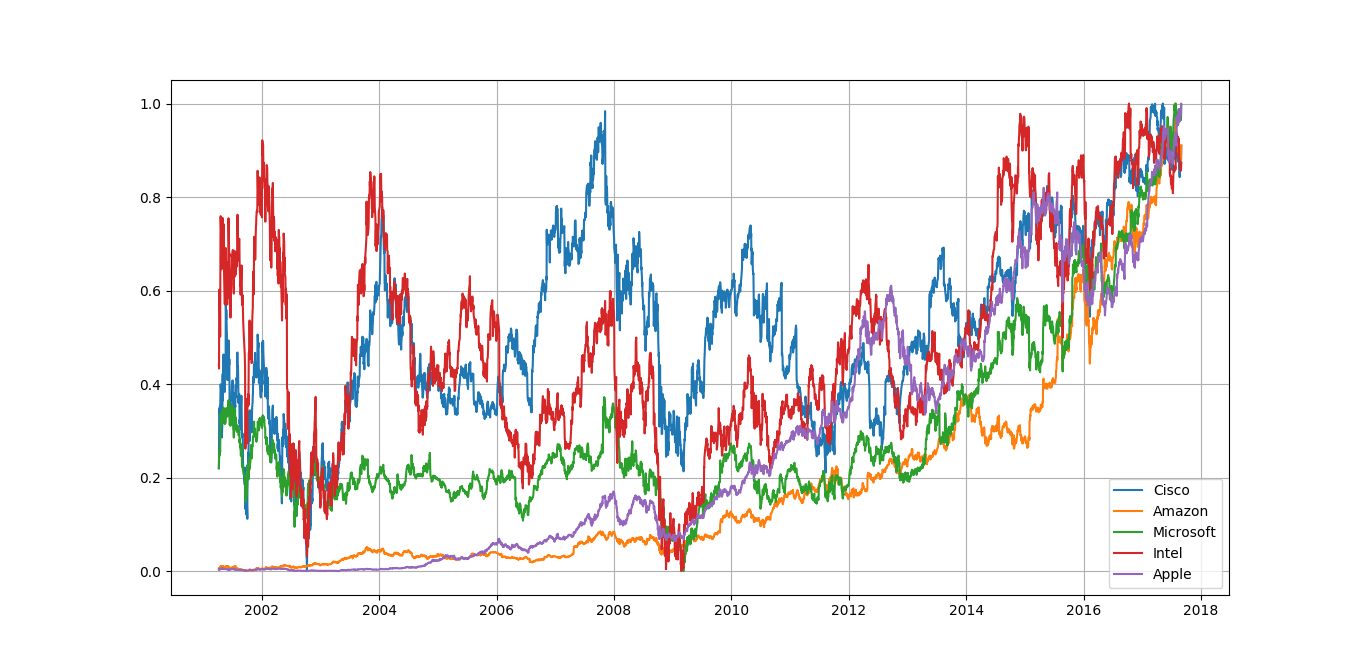
\includegraphics[scale=4]{empresas_normalizado}}
	\caption{Dados normalizados para treinamento}
	\fonte{Elaborado pelo autor}
	\label{exec-intel-coleta}
\end{grafico}

\section{DESENVOLVIMENTO DA REDE NEURAL ARTIFICIAL}
O ambiente de desenvolvimento do modelo de RNA proposto baseou-se nas ferramentas definidas no capítulo anterior, sendo elas a linguagem de programação Python, em sua versão 3.6.0, e a biblioteca PyBrain. Esta Seção detalha todos os procedimentos realizados para a implementação do modelo desenvolvido, evidenciando aspectos gerais de como trabalhar com Python e PyBrain.
\subsection{\textit{Script} para criação de um modelo \textit{FeedForward}}
A implementação de uma RNA com a topologia \textit{FeedForward} foi construída através do módulo pybrain.structure.networks. O mesmo tem como objetivo, especificar como são tratados o fluxo dos dados de entrada da rede. O Código 10 demonstra a importação do módulo e a criação da topologia determinada.

\lstinputlisting[language=Python, label=objeto-feedforward, caption=Construção de uma RNA com a estrutura \textit{FeedForward}]{src/FeedForward.py}

\subsection{Organização das camadas do modelo}
Após a implementação da topologia, faz-se necessário organizar suas camadas, assim como são tratados os respectivos neurônios das mesmas. Para a construção desta etapa, a biblioteca PyBrain oferece, através do módulo pybrain.structure, suporte à inserção via parâmetros, especificando a quantidade de variáveis para cada camada e, também, suas características. No Código 11 é possível observar a classe que implementa o método desenvolvido para a construção das camadas.

\lstinputlisting[language=Python, label=feedforward-layer, caption=Implementação da classe de criação de camadas]{src/feedforward_layers_pybrain.py}

Neste código são importados dois objetos do tipo \textit{Layer}, denominados \textit{LinearLayer} e \textit{SigmoidLayer}. A camada de entrada é composta pelo objeto \textit{LinearLayer}, onde os dados não sofrem nenhuma transformação, apenas transferindo-os para a camada posterior. A camada oculta é composta pelo objeto \textit{SigmoidLayer}, que implementa o cálculo da Equação (3.4) para os dados recebidos. Por fim, a camada oculta também é composta pelo objeto \textit{LinearLayer}, resultando na resposta da rede.   

Realizada a etapa de especificação das camadas e suas respectivas funcionalidades, é necessário adicioná-las, efetivamente, ao modelo de rede. Este procedimento deve ser feito por meio dos métodos \textit{addInputModule}, \textit{addModule} e \textit{addOutputModule}. O Código 12 demonstra a função desenvolvida para a inserção das camadas.

\lstinputlisting[language=Python, label=feedforward-layer, caption=Inserção de camadas em um modelo de RNA]{src/add_modulos.py}

Observando este código, pode-se notar que o mesmo recebe um modelo de rede como parâmetro, faz a inserção através dos respectivos métodos citados anteriormente e retorna a rede com a nova configuração.

A partir disto, a rede precisa identificar quais são as distribuições de conexões referente às camadas inseridas, para determinar o fluxo de trabalho dos dados. Este procedimento é realizado através do objeto \textit{FullConnection}, que determina a ligação entre as camadas. Como o modelo será composto por 3 camadas, faz-se necessário realizar duas conexões, uma entre a camada de entrada e a camada oculta e outra entre a camada oculta e a camada de saída. No Código 13 é demonstrado o método desenvolvido para criar esta funcionalidade.

\lstinputlisting[language=Python, label=feedforward-connection, caption=Conectando as camadas criadas na RNA]{src/conexoes-camadas.py}

Concluída a fase de inserção das conexões, apresentada no Código 13, faz-se necessário inserir os pesos iniciais da rede. Este procedimento é executado através do método \textit{sortModules}, disponbilizado pela biblioteca PyBrain, que adiciona, de forma aleatória, os pesos em um intervalo [-2,2].

\subsection{Treinamento da rede}
Para o desenvolvimento do treinamento a biblioteca PyBrain utiliza dois módulos principais, sendo eles o pybrain.datasets, que é responsável por especificar qual o modelo de aprendizado que a rede trabalha, e, para o caso do aprendizado supervisionado, o módulo pybrain.supervised, que contém os respectivos algoritmos para a presente técnica.

Para mapear uma base de dados de aprendizagem supervisionada com as características desejadas, é necessário utilizar o método \textit{SupervisedDataSet}, onde o mesmo recebe como parâmetro a quantidade de entradas referente à base de dados utilizada e a quantidade de saídas desejadas. Para o presente trabalho, foi instanciada uma base de dados de treino para 8 entradas e 1 saída, seguindo as especificações da Seção 4.5.1.

O Código 14 expõe o desenvolvimento do método que realiza a criação da base de treino.

\lstinputlisting[language=Python, label=base-treino-cod, caption=Construção de uma base de dados para treinamento]{src/base-treino.py}

Observando este código, pode-se notar que as linhas 2 e 3 são responsáveis por importar as dependências das bibliotecas utilizadas. Entre as linhas 5 e 9, é realizada a leitura do arquivo da empresa que foi transferida para a função via parâmetro (nome\_empresa). A linha 11 cria o objeto \textit{SupervisedDataSet} com suas devidas configurações, enquanto a linha 13 consome a base de treino a partir do \textit{DataFrame} sem seus oito últimos dias, que são utilizados para testes. Já a linha 14 inicia o processo de inserção das variáveis do \textit{DataFrame} para a nova base, através do método \textit{addSample}.

Também é possível notar, em relação ao \textit{DataFrame}, que são utilizados os dados normalizados para consumir a base de treinamento. Por fim, a distribuição da camada de saída, encontrada na linha 23, está sendo carregada pelo valor de abertura no dia posterior ao estudado, pelo índice [i + 1], caracterizando, de forma correta, a base de treino para o problema proposto.

Após concluído os procedimentos anteriores, pode-se iniciar, efetivamente, o treinamento da RNA. É importante ressaltar que, neste trabalho, o treino foi executado através do algoritmo \textit{Backpropagation}. O Código 15 demostra, de forma simples, como trabalhar com o algoritmo através da biblioteca PyBrain.

\lstinputlisting[language=Python, label=base-treino-cod, caption=Método de treinamento da RNA através do \textit{Backpropagation}]{src/realizaTreinamento.py}

A função implementada no Código 15, inicia o processo de treino a partir da chamada ao objeto \textit{BackPropTrainer}. Este, por sua vez, recebe alguns parâmetros no momento de sua criação, sendo eles: a rede neural em sí, a base de treinamento e a taxa de aprendizagem (\textit{learning rate}), detalhada na Seção 3.5.1. Segundo \citeonline{haykin2000}, um valor recomendado para o parâmetro \textit{learning rate} é de 0.4 (40\%). No presente trabalho, foi utilizada esta taxa como referência para o treinamento, evidenciada na linha 5 do Código 15. Já o parâmetro \textit{verbose}, auxilia o acompanhamento do erro quadrático médio durante o processo de treinamento, guardando as respectivas variações em um vetor unidimensional.

A partir disto, faz-se necessário realizar a chamada ao método \textit{train}. O mesmo recebe um valor responsável por limitar a quantidade de ciclos (iterações) na qual o modelo é treinado, através da variável \textit{epochs}.

O objeto \textit{NetworkWriter}, encontrado na linha 7, pertence ao pacote tools.customxml, implementando pela biblioteca, que utiliza uma classe que pode receber o estado atual de uma rede treinada e gravá-la em um arquivo \textit{eXtensible Markup Language} (XML). Segundo \citeonline{xml}, o XML foi criado para gerar linguagens de notação para necessidades especiais, de fácil manuseio e portabilidade de sua estrutura. Portanto, tendo em vista a capacidade de exportação da RNA para um arquivo XML, algumas possibilidades são oferecidas, tais como: retreinar a mesma, de forma simplificada, e testá-la quando desejado, sem a necessidade de realizar o processo de treinamento novamente.

A estrutura do arquivo gerado, levando em consideração a exportação realizada pelo Código 15, é demonstrada detalhadamente no Código 16.

\lstinputlisting[language=XML, label=base-treino-cod, caption=Estrutura do arquivo XML de uma RNA]{src/rede-feedforward-intel.xml}

Observando o Código 16, pode-se notar que todas as configurações executadas para construir a rede são armazenadas dentro de suas respectivas características, denominadas \textit{tags}. As \textit{tags} são padronizadas para que, no momento de leitura da RNA, através do objeto \textit{networkReader}, todo o ambiente seja importado de forma correta. Analisando as linhas 3, 6 e 14, por exemplo, é possível notar alguns dos parâmetros inseridos anteriormente na RNA. Além disso, também fica evidente a presença dos pesos sinápticos, entre a camada de entrada e a camada oculta, e, entre a camada oculta e a camada de saída, que são fundamentais para salvar um determinado estado da rede.

Por fim, tendo em vista o refinamento de todas as bases de dados coletadas e da implementação do modelo da RNA, todos os procedimentos necessários para realizar os testes foram desenvolvidos, com base na teoria e especificações dos capítulos anteriores. 
